\section{Medical Trials}

\begin{enumerate}[label=\textbf{\Alph*}.]
    \item A medical study tests a treatment on 100 patients. It is known that there is a 50\% chance that a patient, if untreated, will get better naturally. (Else the patient dies!) The researcher wants to see if the treatment increases the recovery rate. She designs a study to test the treatment: she will test it on 100 patients, and will reject the null hypothesis at the 95\% confidence level if enough patients recover. How many of the 100 patients must survive at the end of the study in order for her to reject the null hypothesis under these conditions?

    Let the number of people who survive be $n$, out of a total $N$. Let the probability of recovery be $p$.

    We have a binomial process here, $L(n|N,p) = \frac{N!}{n!(N-n)!}p^{n}(1-p)^{N-n}$


    $H_0: p=0.5$

    $H_1: p \in [0,1]$

    If we say $N=100$ is large enough such that $-2\ln(\Lambda)$ approximates a $\chi^2$ distribution with 1 degree of freedom (0-dimensional $H_0$ vs 1-dimensional $H_1$) 

    \begin{align*}
        \Lambda(n) &= \frac{\sup_{p \in \{0.5\}} L(n|N,p) }{\sup_{p \in [0,1]} L(n|N,p)} \\
    \end{align*}
    \begin{align*}
        &-2\ln(\Lambda(n)) \\
        &= -2\left[\ln\left(\sup_{p \in \{0.5\}} L(n|N,p)\right) - \ln\left(\sup_{p \in [0,1]} L(n|N,p)\right)\right] \\
        &= -2\left[\ln\left(\frac{N!}{n!(N-n)!}(0.5)^{n}(0.5)^{N-n}\right) - \ln\left(\sup_{p \in [0,1]} \frac{N!}{n!(N-n)!}p^{n}(1-p)^{N-n}\right)\right] \\
        &= -2\left[\ln\left(\frac{N!}{n!(N-n)!}\right) - N\ln(2) - \ln\left(\frac{N!}{n!(N-n)!}\right) - \ln\left(\sup_{p \in [0,1]} p^{n}(1-p)^{N-n}\right)\right] \\
        &= 2\left[N\ln(2) + \sup_{p \in [0,1]} n\ln(p) + (N-n)\ln(1-p)\right] \\
    \end{align*}

    Find that sup by setting the derivative equal to zero:
    \begin{align*}
        0 &= n\frac{1}{p} - (N-n)\frac{1}{1-p} \\
        (N-n)\frac{1}{1-p} &= n\frac{1}{p} \\
        (N-n)p &= n(1-p) \\
        Np-np &= n-np \\
        p &= \frac{n}{N} \\
    \end{align*}


    \begin{align*}
        -2\ln(\Lambda(n)) &= 2\left[N\ln(2) + n\ln(\frac{n}{N}) + (N-n)\ln(1-\frac{n}{N})\right] \\
    \end{align*}

    For a given value of $n$ here we can get a $\chi^2(1)$ value, which lets us get the $p$-value. Here's a plot of $p$-value vs $n$, which has two solutions for $p=0.05$, i.e. We should reject the null hypothesis if either $n < 40$ (the treatment kills people) or $n>60$ (the treatment helps). Assuming the treatment definitely doesn't hurt, then just go with 60.

    \begin{center}
        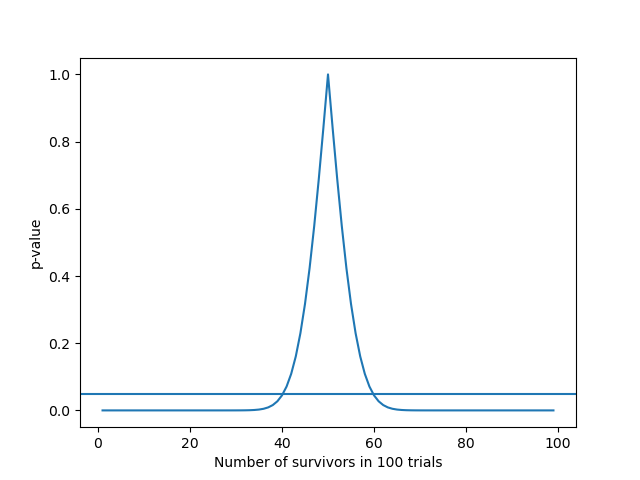
\includegraphics[width=\textwidth]{q1_a.png}
    \end{center}

    See the code for details on the calculation of these numbers, but I just calculated the $p$-value for increasing $n$ until it went below 0.05 (95\% confidence level).

    \item Her hospital's medical ethics board advises her that if the treatment proves to be very effective, then it would be unethical to continue the study. Instead, she should end the study early and publish the results so that other patients can benefit from the treatment. Therefore she modifies the study. Starting after the first 25 patients are treated, she counts up how many patients have recovered, and calculates the probability that at least that many would have recovered just by chance. If this probability is less than 1\%, she will end the study immediately and reject the null hypothesis, concluding that the treatment is effective. She continues to calculate this probability after each additional patient is treated until the treatment has proven effective or until she has treated 100 patients. The treatment is deemed successful if either the study ended early due to its apparent effectiveness, or if after 100 patients the number of recovered patients is greater than that calculated in Part A. In these two cases she will either write a paper saying that the treatment proved effective at the 99\% CL or at the 95\% CL, depending on whether the trial ended early or not. Suppose that in reality the treatment has no effect on patient outcomes. What is the probability that the null hypothesis is rejected anyway? What is the probability that researcher publishes a paper rejecting the null hypothesis at the 99\% CL?
    
    Simulate this: 




\end{enumerate}
